\documentclass[tikz,border=10pt]{standalone}
\usepackage{tikz}
\usetikzlibrary{shapes.geometric,arrows.meta,positioning,fit,backgrounds,shadows,decorations.pathreplacing}

\begin{document}
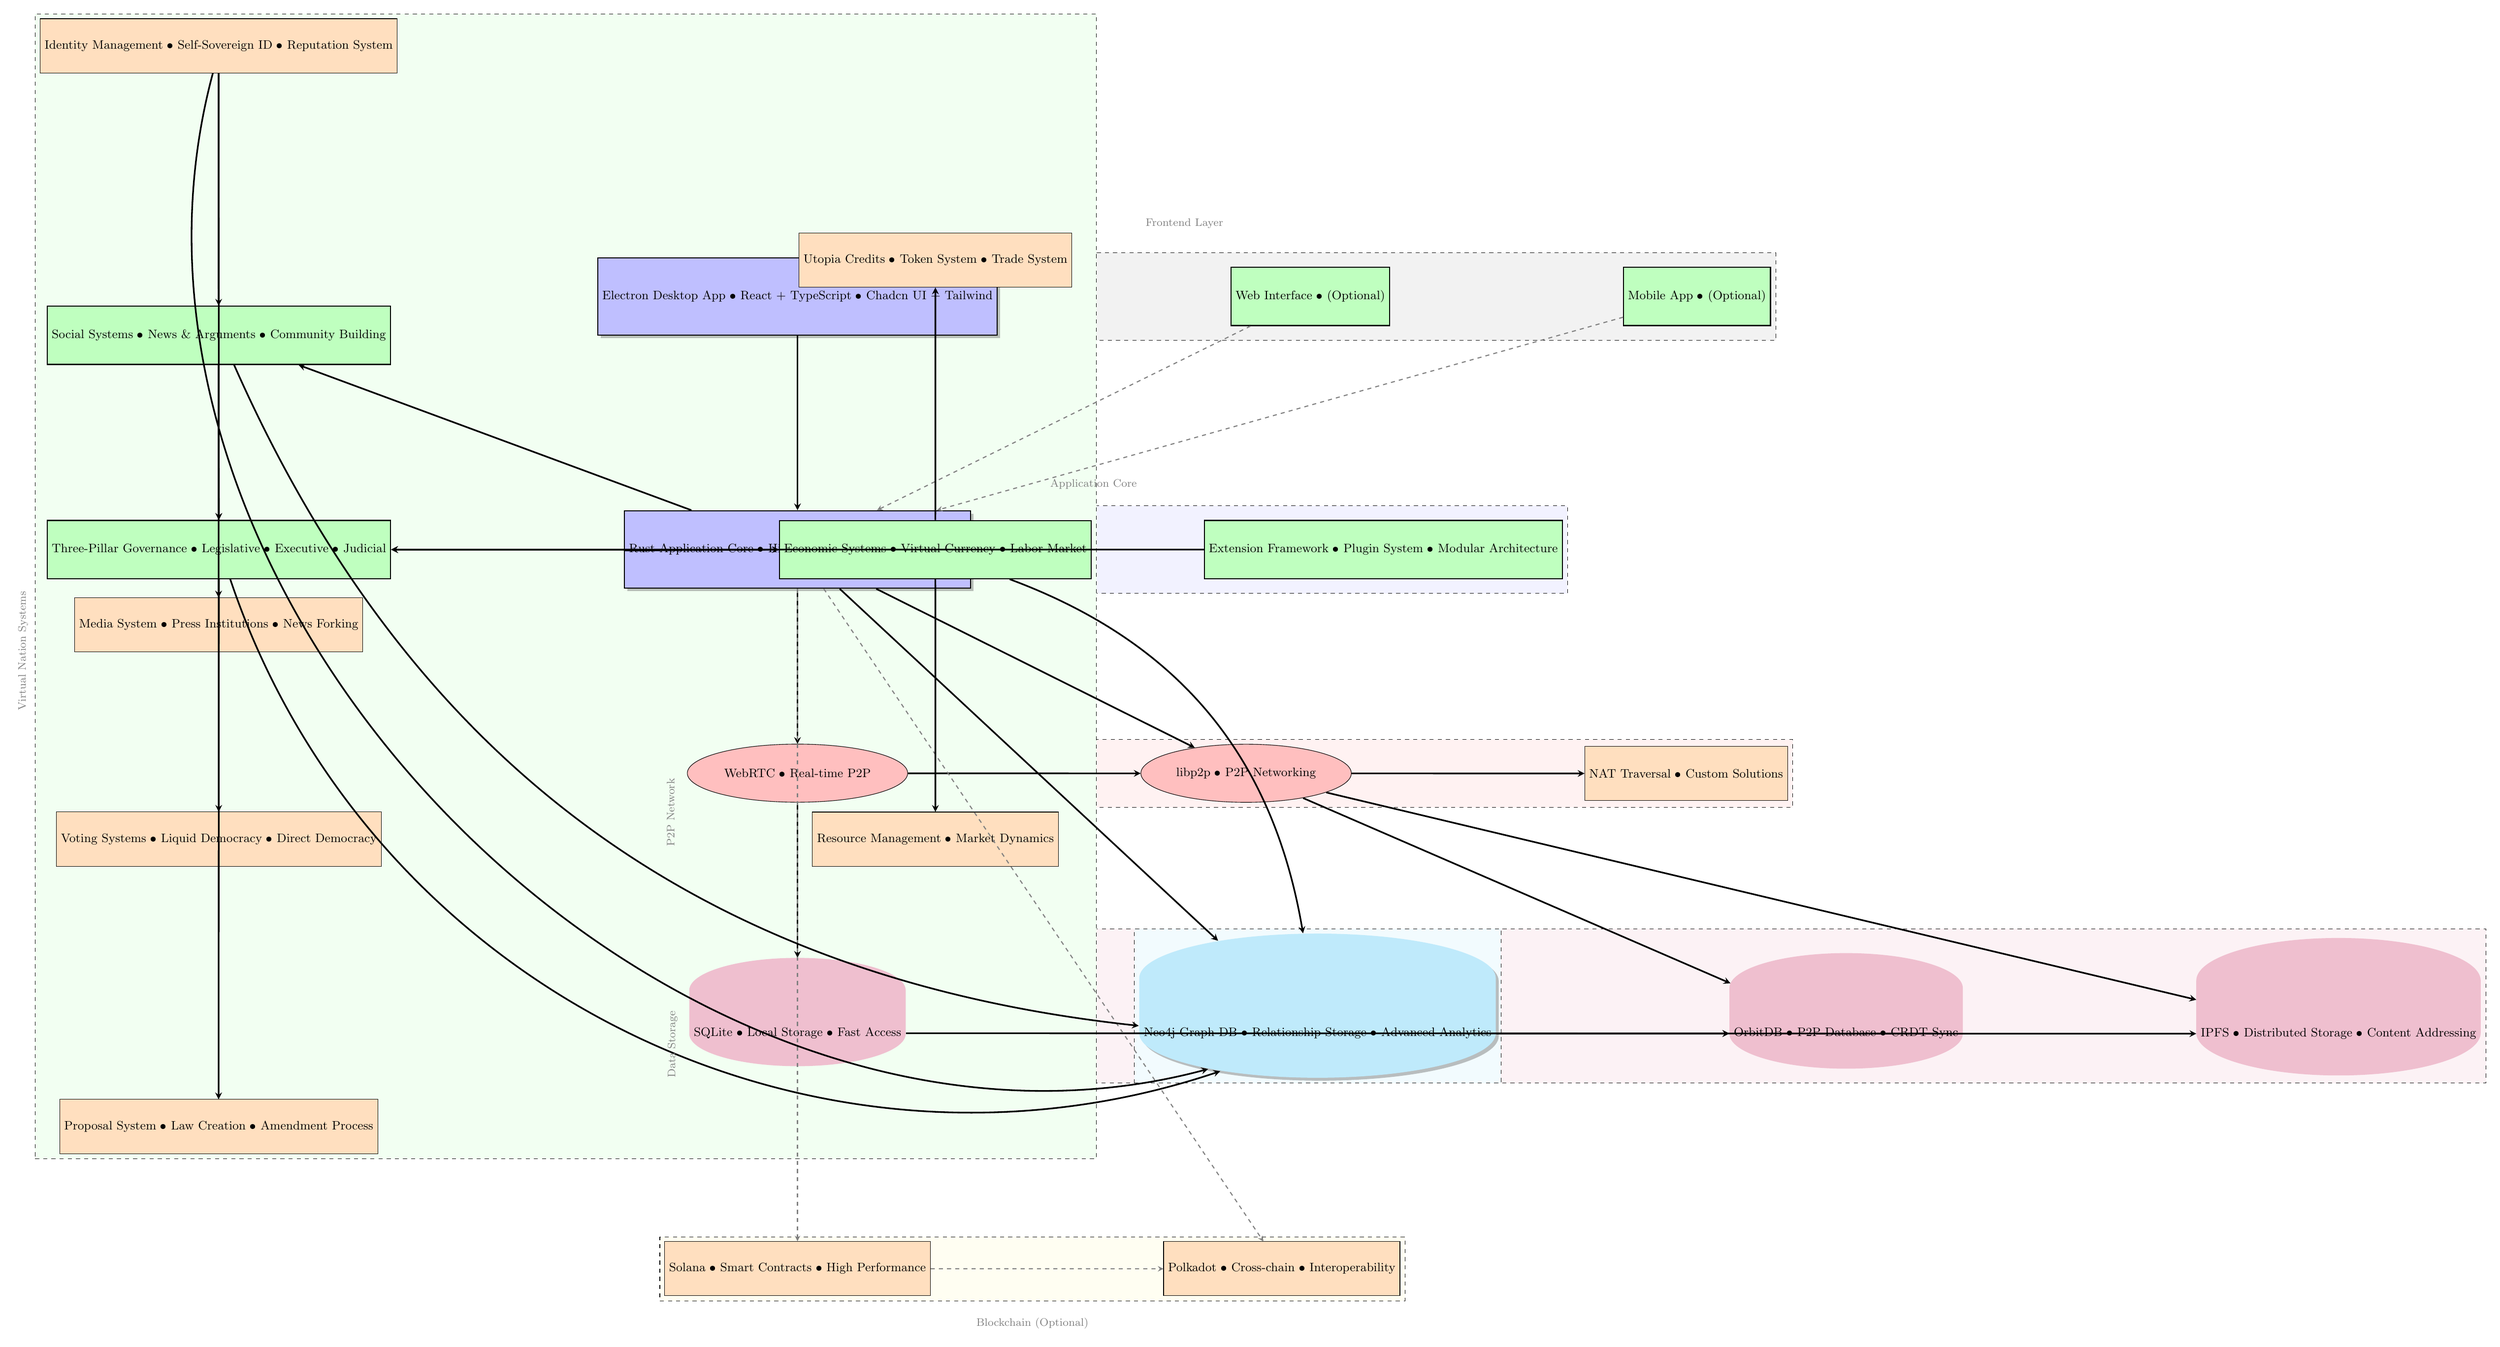
\begin{tikzpicture}[scale=2.5,
    node distance=6cm,
    every node/.style={font=\small},
    % Main components - Enhanced sizing
    core/.style={rectangle,draw,minimum width=3.5cm,minimum height=2cm,fill=blue!25,thick,drop shadow},
    layer/.style={rectangle,draw,minimum width=3cm,minimum height=1.5cm,fill=green!25,thick},
    service/.style={rectangle,draw,minimum width=2.8cm,minimum height=1.4cm,fill=orange!25},
    storage/.style={cylinder,shape border rotate=90,aspect=0.3,minimum height=1.6cm,minimum width=2.8cm,fill=purple!25},
    network/.style={ellipse,draw,minimum width=3cm,minimum height=1.5cm,fill=red!25},
    graphdb/.style={cylinder,shape border rotate=90,aspect=0.25,minimum height=1.8cm,minimum width=3cm,fill=cyan!25,thick,drop shadow},
    arrow/.style={->,>=stealth,very thick},
    dashed_arrow/.style={->,>=stealth,dashed,gray,thick}
]

% Frontend Layer
\node[core] (electron) {Electron Desktop App • React + TypeScript • Chadcn UI + Tailwind};
\node[layer,right=of electron] (web) {Web Interface • (Optional)};
\node[layer,right=of web] (mobile) {Mobile App • (Optional)};

% Core Application Layer
\node[core,below=4.5cm of electron] (rust_core) {Rust Application Core • High Performance • Memory Safety};
\node[layer,right=of rust_core] (extension_framework) {Extension Framework • Plugin System • Modular Architecture};

% P2P Communication Layer
\node[network,below=4cm of rust_core] (webrtc) {WebRTC • Real-time P2P};
\node[network,right=of webrtc] (libp2p) {libp2p • P2P Networking};
\node[service,right=of libp2p] (nat_traversal) {NAT Traversal • Custom Solutions};

% Storage Layer
\node[storage,below=4cm of webrtc] (sqlite) {SQLite • Local Storage • Fast Access};
\node[graphdb,right=of sqlite] (neo4j) {Neo4j Graph DB • Relationship Storage • Advanced Analytics};
\node[storage,right=of neo4j] (orbitdb) {OrbitDB • P2P Database • CRDT Sync};
\node[storage,right=of orbitdb] (ipfs) {IPFS • Distributed Storage • Content Addressing};

% Blockchain Layer (Optional)
\node[service,below=4.5cm of sqlite] (solana) {Solana • Smart Contracts • High Performance};
\node[service,right=of solana] (polkadot) {Polkadot • Cross-chain • Interoperability};

% Governance Systems
\node[layer,left=6cm of rust_core] (governance) {Three-Pillar Governance • Legislative • Executive • Judicial};
\node[service,below=of governance] (voting) {Voting Systems • Liquid Democracy • Direct Democracy};
\node[service,below=of voting] (proposals) {Proposal System • Law Creation • Amendment Process};

% Social Systems
\node[layer,above=4cm of governance] (social) {Social Systems • News \& Arguments • Community Building};
\node[service,above=of social] (identity) {Identity Management • Self-Sovereign ID • Reputation System};
\node[service,below=of social] (media) {Media System • Press Institutions • News Forking};

% Economic Systems
\node[layer,right=10cm of governance] (economy) {Economic Systems • Virtual Currency • Labor Market};
\node[service,above=of economy] (currency) {Utopia Credits • Token System • Trade System};
\node[service,below=of economy] (resources) {Resource Management • Market Dynamics};

% Background groupings
\begin{scope}[on background layer]
\node[fill=gray!10,draw,dashed,fit=(electron)(web)(mobile)] (frontend_group) {};
\node[fill=blue!5,draw,dashed,fit=(rust_core)(extension_framework)] (core_group) {};
\node[fill=red!5,draw,dashed,fit=(webrtc)(libp2p)(nat_traversal)] (network_group) {};
\node[fill=purple!5,draw,dashed,fit=(sqlite)(neo4j)(orbitdb)(ipfs)] (storage_group) {};
\node[fill=cyan!5,draw,dashed,fit=(neo4j)] (graph_group) {};
\node[fill=yellow!5,draw,dashed,fit=(solana)(polkadot)] (blockchain_group) {};
\node[fill=green!5,draw,dashed,fit=(governance)(voting)(proposals)(social)(identity)(media)(economy)(currency)(resources)] (systems_group) {};
\end{scope}

% Connections - Frontend to Core
\draw[arrow] (electron) -- (rust_core);
\draw[dashed_arrow] (web) -- (rust_core);
\draw[dashed_arrow] (mobile) -- (rust_core);

% Core to Systems
\draw[arrow] (rust_core) -- (governance);
\draw[arrow] (rust_core) -- (social);
\draw[arrow] (rust_core) -- (economy);
\draw[arrow] (extension_framework) -- (governance);

% Network Layer connections
\draw[arrow] (rust_core) -- (webrtc);
\draw[arrow] (rust_core) -- (libp2p);
\draw[arrow] (webrtc) -- (libp2p);
\draw[arrow] (libp2p) -- (nat_traversal);

% Storage connections
\draw[arrow] (webrtc) -- (sqlite);
\draw[arrow] (rust_core) -- (neo4j);
\draw[arrow] (libp2p) -- (orbitdb);
\draw[arrow] (libp2p) -- (ipfs);
\draw[arrow] (sqlite) -- (orbitdb);
\draw[arrow] (neo4j) -- (orbitdb);
\draw[arrow] (neo4j) -- (ipfs);

% Blockchain connections
\draw[dashed_arrow] (rust_core) -- (solana);
\draw[dashed_arrow] (rust_core) -- (polkadot);
\draw[dashed_arrow] (solana) -- (polkadot);

% System interconnections
\draw[arrow] (governance) -- (voting);
\draw[arrow] (governance) -- (proposals);
\draw[arrow] (identity) -- (social);
\draw[arrow] (social) -- (media);
\draw[arrow] (economy) -- (currency);
\draw[arrow] (economy) -- (resources);

% Cross-system connections
\draw[arrow] (identity) -- (governance);
\draw[arrow] (social) -- (governance);
\draw[arrow] (economy) -- (governance);

% Graph database connections to governance systems
\draw[arrow] (governance) to[bend right=45] (neo4j);
\draw[arrow] (social) to[bend right=30] (neo4j);
\draw[arrow] (economy) to[bend left=30] (neo4j);
\draw[arrow] (identity) to[bend right=60] (neo4j);

% Labels
\node[above=0.5cm of frontend_group,font=\footnotesize,text=gray] {Frontend Layer};
\node[above=0.3cm of core_group,font=\footnotesize,text=gray] {Application Core};
\node[left=0.3cm of network_group,font=\footnotesize,text=gray,rotate=90] {P2P Network};
\node[left=0.3cm of storage_group,font=\footnotesize,text=gray,rotate=90] {Data Storage};
\node[below=0.3cm of blockchain_group,font=\footnotesize,text=gray] {Blockchain (Optional)};
\node[left=0.3cm of systems_group,font=\footnotesize,text=gray,rotate=90] {Virtual Nation Systems};

\end{tikzpicture}
\end{document}
